\documentclass[
coverheight=9in,
coverwidth=6in,
spinewidth=0.4745in,
bleedwidth=.125in,
marklength=0in,
markcolor=black]{bookcover}

\usepackage{fontspec}

\setmainfont{Libertinus Serif}
\newfontface{\glagoliticA}{Menaion Unicode}


\newbookcoverpart{pfront}{
\setpartposx{\marklength+\bleedwidth+\spinewidth+\coverwidth+4mm}
\setpartposy{\marklength+\bleedwidth+10mm}\setpartheight{\coverheight-20mm}
\setpartwidth{\coverwidth-20mm}
\settrimmedpart{0mm}{0mm}{0pt}{0pt}
}

\newbookcoverpart{pback}{
\setpartposx{\marklength+\bleedwidth+10mm}
\setpartposy{\marklength+\bleedwidth+10mm}\setpartheight{\coverheight-20mm}
\setpartwidth{\coverwidth-15mm}
\settrimmedpart{0mm}{0mm}{0pt}{0pt}
}

\begin{document}

\begin{bookcover}

\bookcovercomponent{center}{bg whole}{\hspace*{-10mm}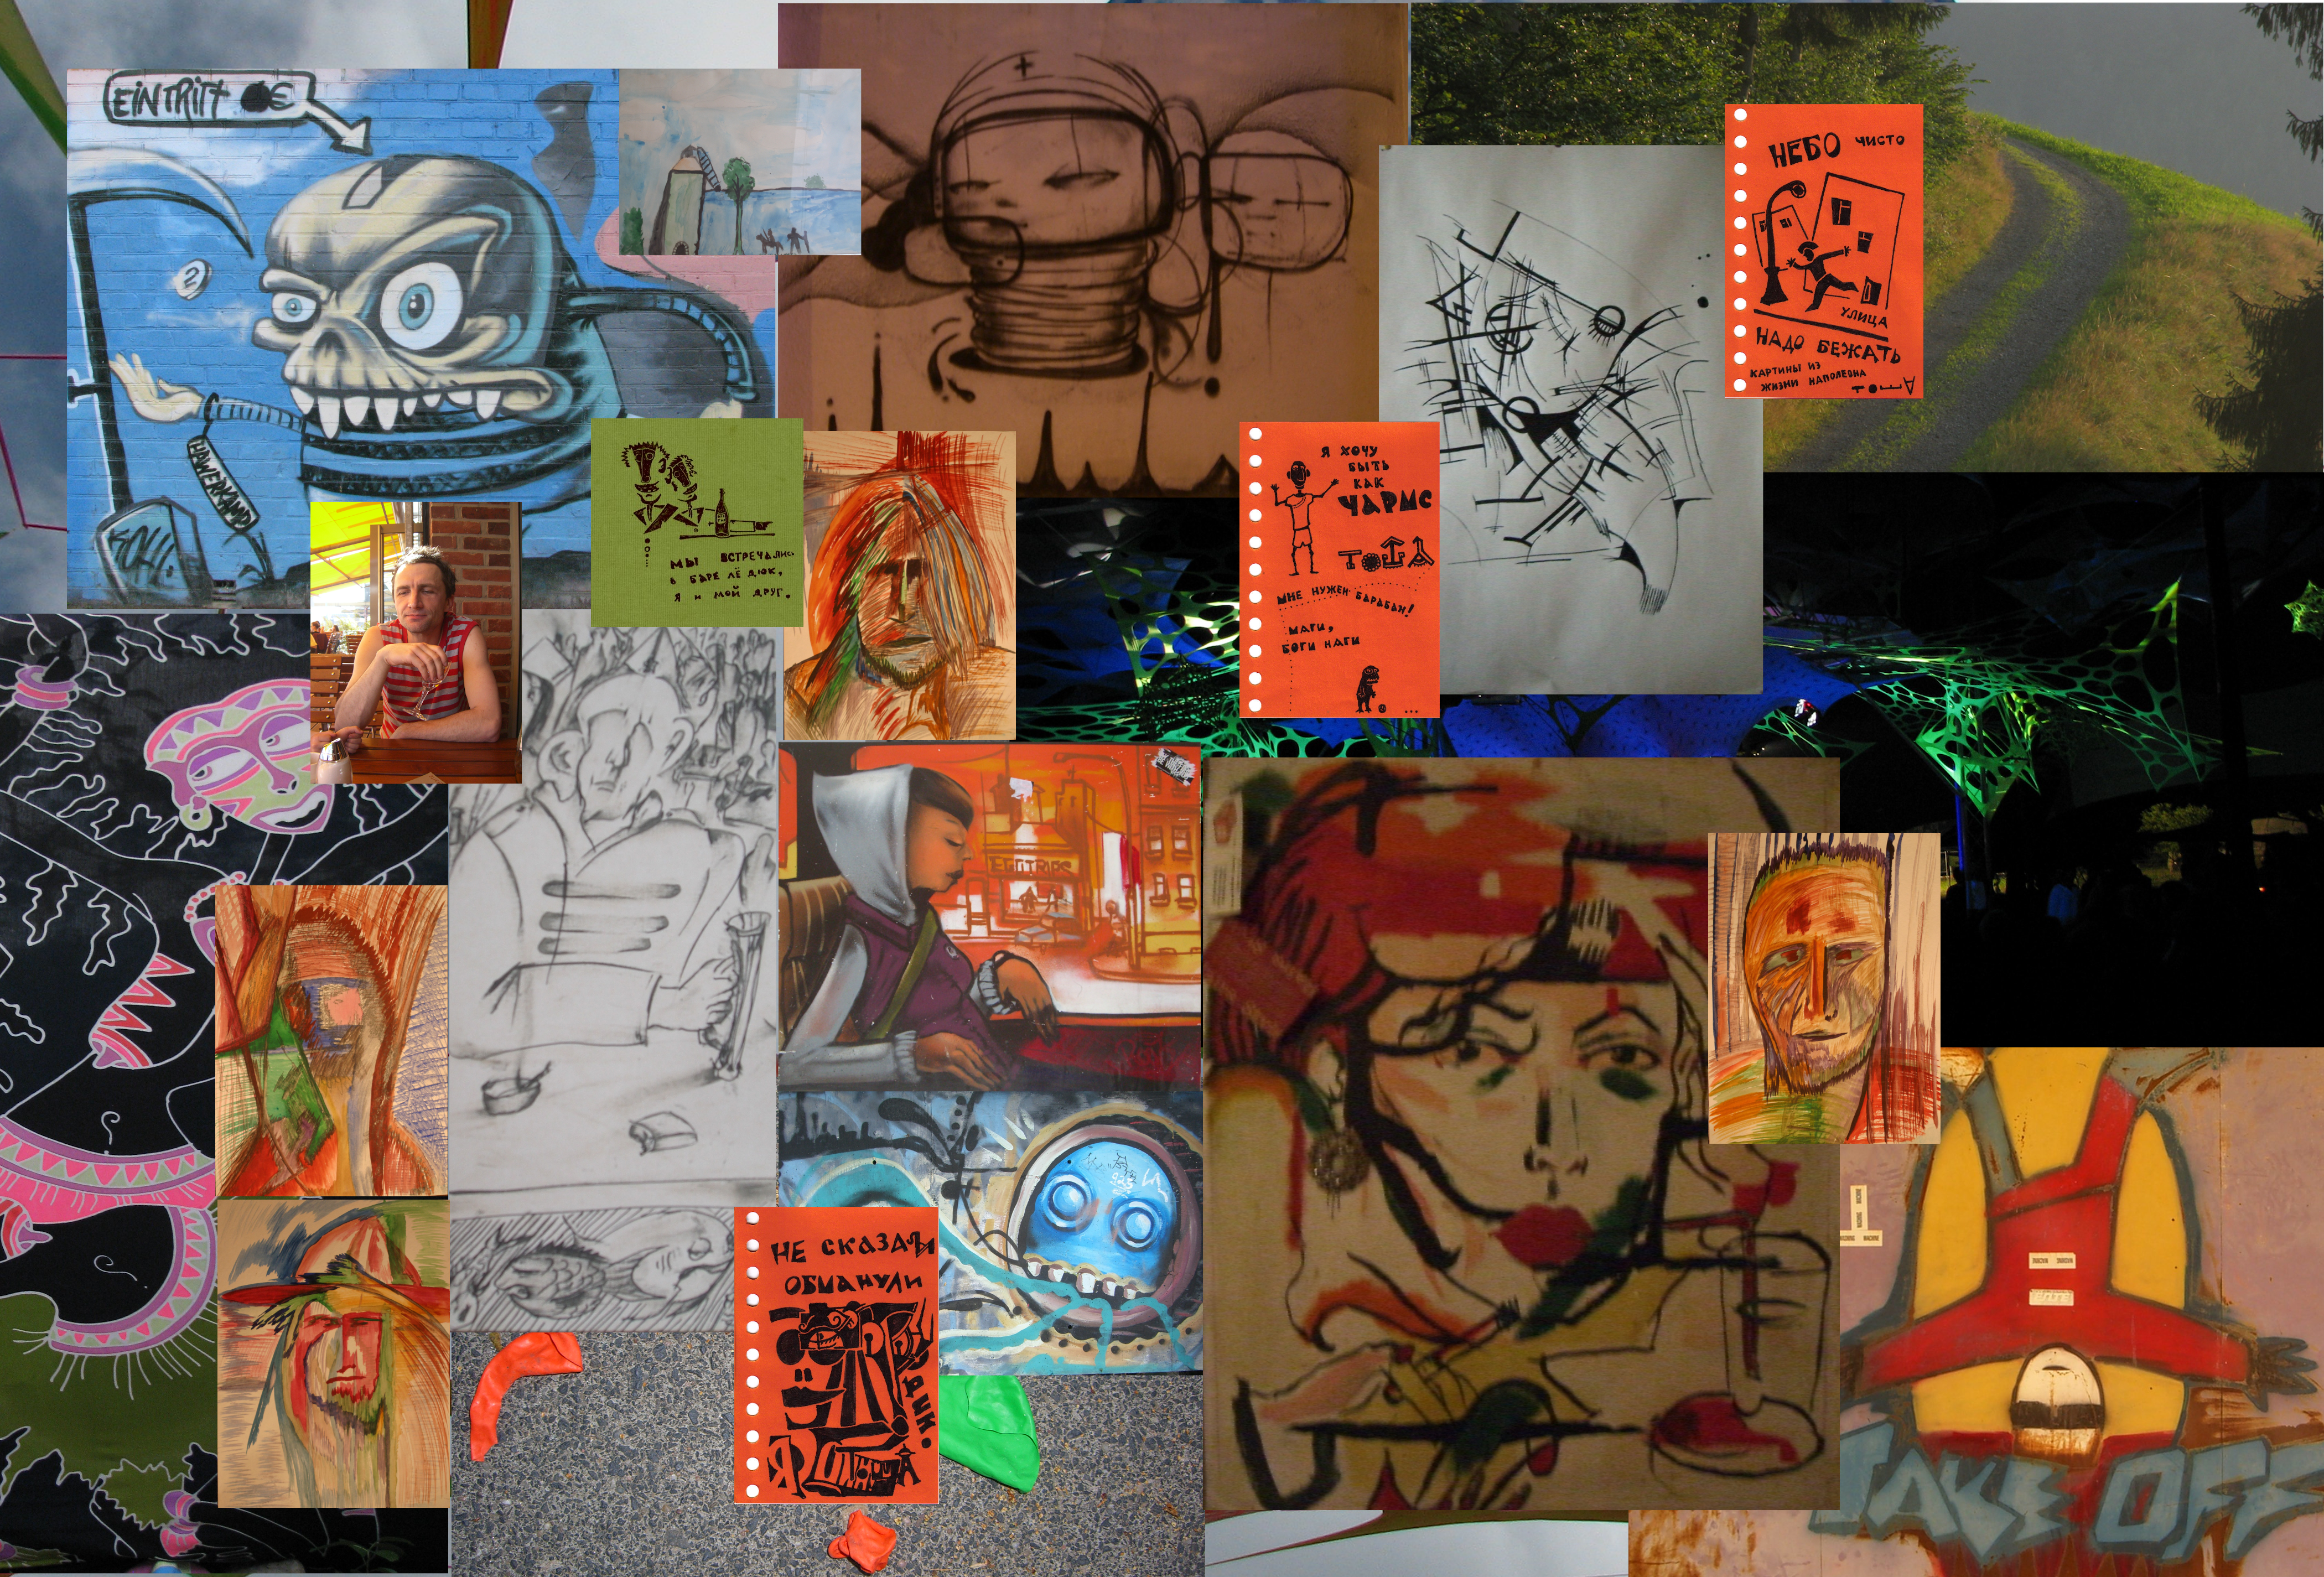
\includegraphics[height=\coverheight+\bleedwidth+\bleedwidth]{fon}}

\bookcovercomponent{center}{spine}
{\rotatebox[origin=c]{90}{
\color{white}\fontsize{18}{25}\usefont{OT1}{lmtt}{b}{n}
\qquad\qquad\qquad\qquad{\glagoliticA ⰒⰋⰔⰠⰏⰀ ⰛⰀⰔⰕⰠⰡ}
}}

\bookcovercomponent{center}{pfront}{
\begin{flushright}
\vskip57mm
{\color{white}\fontsize{30}{30}\usefont{OT1}{lmtt}{b}{n}
{\glagoliticA ⰒⰋⰔⰠⰏⰀ\\ⰛⰀⰔⰕⰠⰡ}\\
}
\vfill
\ \\
\end{flushright}
}

\bookcovercomponent{center}{pback}{
\begin{flushleft}
\end{flushleft}
}


\end{bookcover}

\end{document}
